%%%%%%%%%%%%%%%%%%%%%%%%%%%%%%%%%%%%%%%%%
% Beamer Presentation
% LaTeX Template
% Version 1.0 (10/11/12)
%
% This template has been downloaded from:
% http://www.LaTeXTemplates.com
%
% License:
% CC BY-NC-SA 3.0 (http://creativecommons.org/licenses/by-nc-sa/3.0/)
%
%%%%%%%%%%%%%%%%%%%%%%%%%%%%%%%%%%%%%%%%%

%----------------------------------------------------------------------------------------
%	PACKAGES AND THEMES
%----------------------------------------------------------------------------------------

\documentclass{beamer}

\mode<presentation> {

% The Beamer class comes with a number of default slide themes
% which change the colors and layouts of slides. Below this is a list
% of all the themes, uncomment each in turn to see what they look like.

%\usetheme{default}
%\usetheme{AnnArbor}
%\usetheme{Antibes}
%\usetheme{Bergen}
%\usetheme{Berkeley}
%\usetheme{Berlin}
%\usetheme{Boadilla}
%\usetheme{CambridgeUS}
%\usetheme{Copenhagen}
%\usetheme{Darmstadt}
%\usetheme{Dresden}
%\usetheme{Frankfurt}
%\usetheme{Goettingen}
%\usetheme{Hannover}
%\usetheme{Ilmenau}
%\usetheme{JuanLesPins}
%\usetheme{Luebeck}
%\usetheme{Madrid}
%\usetheme{Malmoe}
%\usetheme{Marburg}
%\usetheme{Montpellier}
%\usetheme{PaloAlto}
\usetheme{Pittsburgh}
%\usetheme{Rochester}
%\usetheme{Singapore}
%\usetheme{Szeged}
%\usetheme{Warsaw}

% As well as themes, the Beamer class has a number of color themes
% for any slide theme. Uncomment each of these in turn to see how it
% changes the colors of your current slide theme.

%\usecolortheme{albatross}
%\usecolortheme{beaver}
%\usecolortheme{beetle}
%\usecolortheme{crane}
%\usecolortheme{dolphin}
%\usecolortheme{dove}
%\usecolortheme{fly}
%\usecolortheme{lily}
%\usecolortheme{orchid}
%\usecolortheme{rose}
%\usecolortheme{seagull}
%\usecolortheme{seahorse}
%\usecolortheme{whale}
%\usecolortheme{wolverine}

%\setbeamertemplate{footline} % To remove the footer line in all slides uncomment this line
%\setbeamertemplate{footline}[page number] % To replace the footer line in all slides with a simple slide count uncomment this line

%\setbeamertemplate{navigation symbols}{} % To remove the navigation symbols from the bottom of all slides uncomment this line
}

\usepackage{graphicx} % Allows including images
\usepackage{booktabs} % Allows the use of \toprule, \midrule and \bottomrule in tables

%----------------------------------------------------------------------------------------
%	TITLE PAGE
%----------------------------------------------------------------------------------------

\title[BHD]{Boston Housing Regression Analysis} % The short title appears at the bottom of every slide, the full title is only on the title page

\author{Liping Gu, Zhezhi Hou, Ahmad Jarara} % Your name
\institute[BU] % Your institution as it will appear on the bottom of every slide, may be shorthand to save space
{
Binghamton University \\ % Your institution for the title page
\medskip
%\textit{} % Your email address
}
\date{\today} % Date, can be changed to a custom date

\begin{document}

\begin{frame}
\titlepage % Print the title page as the first slide
\end{frame}

\begin{frame}
\frametitle{Overview} % Table of contents slide, comment this block out to remove it
\tableofcontents % Throughout your presentation, if you choose to use \section{} and \subsection{} commands, these will automatically be printed on this slide as an overview of your presentation
\end{frame}

\begin{frame}
\section{High Level Overview}
\frametitle{High Level Overview}
\begin{itemize}
\item Variable Analysis
\item Model Trimming
\item Featured Variables
\item Neighborhood Analysis
\item Model Selection
\end{itemize}
\end{frame}


%\subsection{Variable Analysis}
\begin{frame}
\frametitle{Variable Analysis}
\begin{itemize}
\item 1stFlrSF
\item 2ndFlrSF
\item WoodDeckSF
\item OpenPorchSF
\item YearBuilt
\item BsmtSF
\item Neighborhood
\item Street
\end{itemize}
\end{frame}


%\subsection{Model trimming}
\begin{frame}
\frametitle{Model trimming}

We eliminate the Street attribute from our model.\\~\\

The aim of this analysis is not to overfit the formula to the little data we have, but instead have our model be the best at accurately predicting new elements. 
\end{frame}

%\subsection{Featured Variables}
\begin{frame}
\frametitle{Featured Variables}
\begin{itemize}
\item X2ndFlrSF
\item WoodDeckSF
\item OpenPorchSF
\item BasementSF
\end{itemize}
\end{frame}

%\subsection{Neighborhood Analysis}
\begin{frame}
\frametitle{Model trimming}

Special emphasis on neighborhood.\\~\\

This removes degrees of freedom from the analysis and allows for more emphasis on other attributes.

However, this methodology is significantly flawed!
\end{frame}

%\subsection{Model Selection}
\begin{frame}
\frametitle{Model Selection}

Very small sample size suggests a lax model.\\~\\

Pitfalls of a complex analysis:
\begin{itemize}
  \item Rigid model
  \item Simpson's Paradox
\end{itemize}
  
Then a simple linear regression is most likely the correct one.
\end{frame}


\begin{frame}
\section{Model Instantiation}
\frametitle{Model Instantiation}
\begin{itemize}
\item Initial Linear Regression Model
\item Neighborhood Segregation
\item Correlation Study
\item Applying Transformations
\item Intermediary Models and Stepwise Analysis
\item Final Model
\end{itemize}
\end{frame}

\begin{frame}
\frametitle{Initial Linear Regression Model}
\begin{figure}
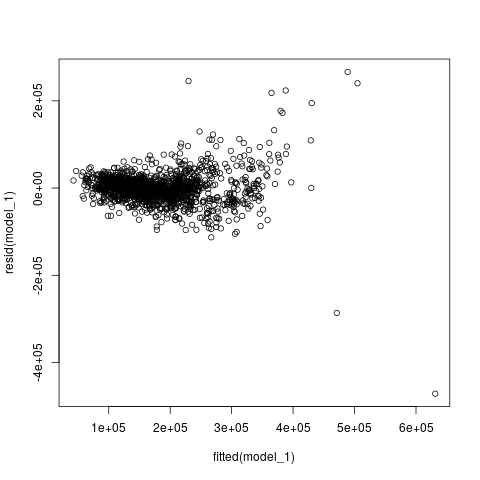
\includegraphics[width=0.75\linewidth,keepaspectratio=true]{img/heteroscedastic.png}
\end{figure}
\end{frame}

\begin{frame}
\frametitle{Neighborhood Segregation}
\begin{table}
\begin{tabular}{l l l}
\toprule
\textbf{Neighborhood} & \textbf{Count} & \textbf{mean(SalePrice)}\\
\midrule
NAmes        &   225 &        145847.1 \\
CollgCr      &   150 &        197965.8 \\
OldTown      &   113 &        128225.3 \\
NWAmes       &    73 &        189050.1 \\
Timber       &    38 &        242247.4 \\
IDOTRR       &    37 &        100123.8 \\
ClearCr      &    28 &        212565.4 \\
StoneBr      &    25 &          310499 \\
SWISU        &    25 &        142591.4 \\
Blmngtn      &    17 &        194870.9 \\
MeadowV      &    17 &        98576.47 \\
NPkVill      &     9 &        142694.4 \\
Blueste      &     2 &          137500 \\
\bottomrule
\end{tabular}
\caption{(Omission of other neighborhoods for brevity)}
\end{table}
\end{frame}


\begin{frame}
\frametitle{Neighborhood Segregation Pt. 2}
\begin{figure}
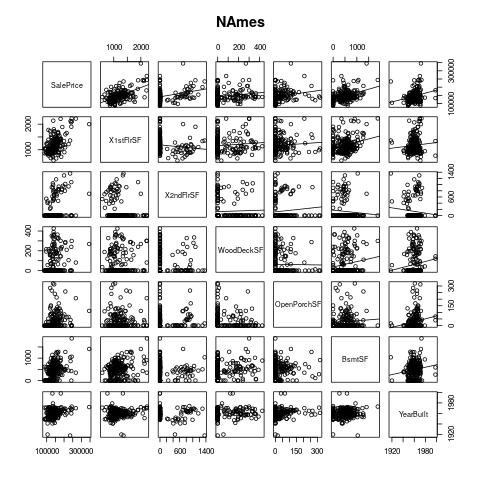
\includegraphics[width=0.75\linewidth,keepaspectratio=true]{img/pairNAmes.png}
\end{figure}
\end{frame}

\begin{frame}
\frametitle{Neighborhood Segregation Pt. 2}
\begin{figure}
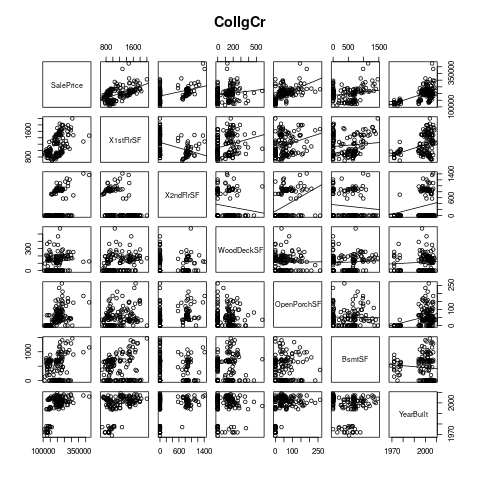
\includegraphics[width=0.75\linewidth,keepaspectratio=true]{img/pairCollgCr.png}
\end{figure}
\end{frame}

\begin{frame}
\frametitle{Neighborhood Segregation Pt. 2}
\begin{figure}
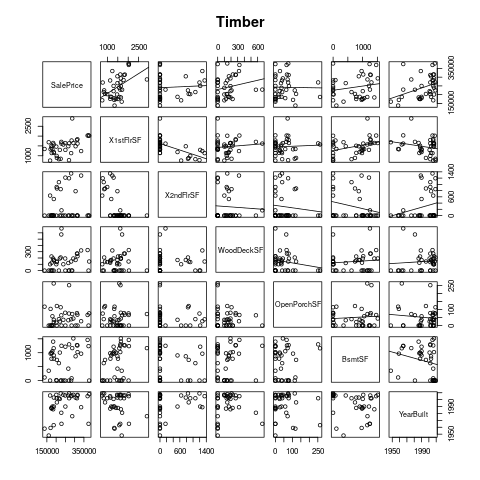
\includegraphics[width=0.75\linewidth,keepaspectratio=true]{img/pairTimber.png}
\end{figure}
\end{frame}


\begin{frame}
\Huge{\centerline{Ignore all that craziness...}}
\end{frame}


\begin{frame}
\frametitle{Correlation Study}
\begin{figure}
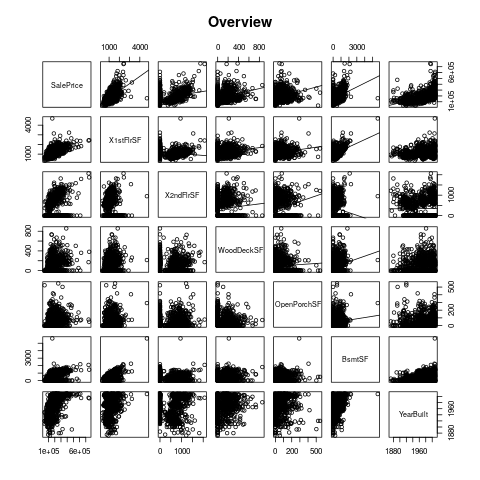
\includegraphics[width=0.75\linewidth,keepaspectratio=true]{img/overview.png}
\end{figure}
\end{frame}


\begin{frame}
\frametitle{Pesky Heteroscedasticity}
\begin{itemize}
\item Removing neighborhoods stands to lose too much
\item Large amount of variance means an inaccurate regression.
\item  Solution? Apply log transform!
\end{itemize}
\end{frame}

\begin{frame}
\frametitle{Applying Transformations}
\begin{figure}
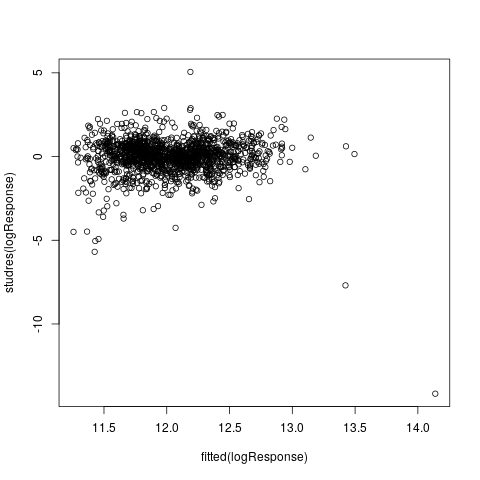
\includegraphics[width=0.75\linewidth,keepaspectratio=true]{img/regOverview.png}
\end{figure}
\end{frame}

\begin{frame}
  \frametitle{Applying Transformations Pt. 2}
  The residuals do not follow normal distribution. \\~\\
  The solution to this is to use the generalized least squares estimator to establish correlation and coefficients for our model.\\~\\
  We do this by applying the weight of $1/\epsilon_i^2$.
  
  \end{frame}


  \begin{frame}
\frametitle{Applying Transformations Pt. 3}
\begin{figure}
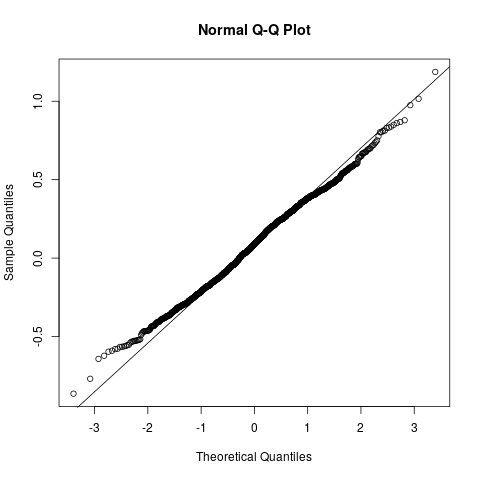
\includegraphics[width=0.75\linewidth,keepaspectratio=true]{img/weightedModel.png}
\end{figure}
\end{frame}

\begin{frame}
\frametitle{Applying Transformations Pt. 4}
\begin{figure}
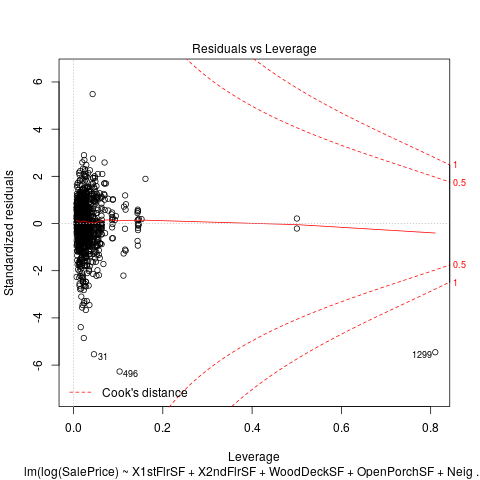
\includegraphics[width=0.75\linewidth,keepaspectratio=true]{img/outincrvl.png}
\end{figure}
\end{frame}

\begin{frame}
\frametitle{Intermediary Models and Stepwise Analysis}
Relevant variables include:
\begin{itemize}
\item X1stFlrSF
\item X2ndFlrSF
\item WoodDeckSF
\item BsmtSF
\item YearBuilt
\end{itemize}
We observed a strong quadratic trend in our correlation analysis, so we included X1stFlrSF$^2$ in our model.\\
Further, we used a stepAIC in both directions, and the only variable it came up with was an interaction variable between the first and second floors. We used that as well.
\end{frame}


\begin{frame}
\frametitle{Final Model}
\begin{table}
\begin{tabular}{l l l}
\toprule
\textbf{Attribute} & \textbf{Coefficient}\\
\midrule
 X1stFlrSF           &  0.0008023042 \\
 X2ndFlrSF           &  0.0005162776 \\
 WoodDeckSF          &   0.000210046 \\
 OpenPorchSF         &  0.0003655512 \\
 BsmtSF              &  0.0001368659 \\
 YearBuilt           &   0.004020196 \\
 X1stFlrSF$^2$         & -1.173194e-07 \\
 X1stFlrSF:X2ndFlrSF & -1.504619e-07 \\
\bottomrule
\end{tabular}
\caption{Neighborhoods omitted for brevity}
\end{table}
\end{frame}



\begin{frame}
\section{Model Verification}
\frametitle{Model Verification}
\begin{itemize}
  \item Predictions
\item Graphical Confirmation
\item Cross Validation
\item Additional Musings
\end{itemize}
\end{frame}


\begin{frame}
\frametitle{Predictions}
\begin{figure}
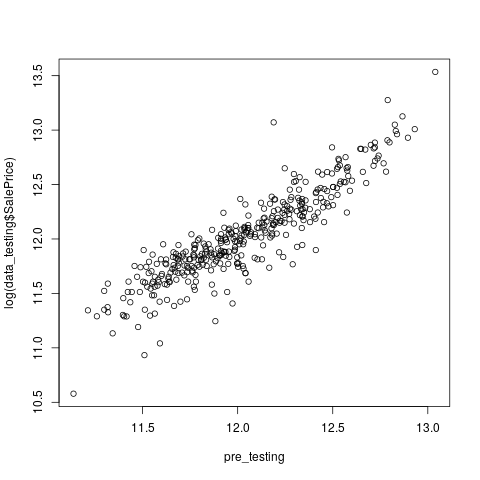
\includegraphics[width=0.75\linewidth,keepaspectratio=true]{img/residTesting.png}
\end{figure}
\end{frame}

\begin{frame}
\Huge{\centerline{Drumroll...}}
\end{frame}

\begin{frame}
\frametitle{Cross Validation}
\begin{figure}
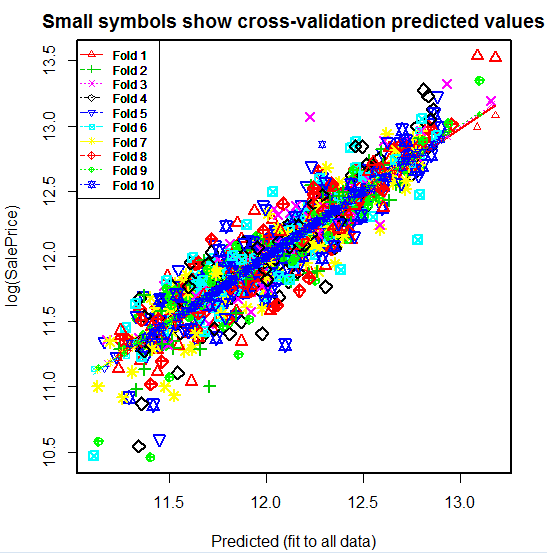
\includegraphics[width=0.75\linewidth,keepaspectratio=true]{img/crossValidation.png}
\end{figure}
\end{frame}

\begin{frame}
  \frametitle{Additional Musings}
  Training data proportionally selected from neighborhood
\begin{itemize}
\item Is there a better model by selecting by neighborhood?
\item No guarantees without guarantees
\end{itemize}
\end{frame}

  \begin{frame}
\frametitle{Outlier Treatment}
\begin{figure}
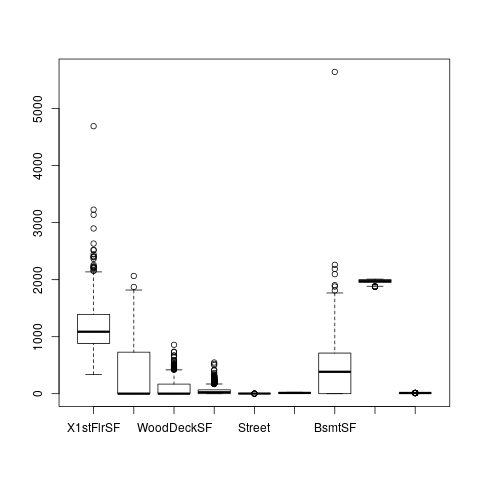
\includegraphics[width=0.75\linewidth,keepaspectratio=true]{img/outlierboxplot.png}
\end{figure}
\end{frame}


 \begin{frame}
 \frametitle{Outlier Treatment Pt. 2}
 \begin{table}
 \begin{tabular}{l l l l}
 \toprule
 \textbf{Parameter} & \textbf{Old Coef} & \textbf{New Coef} & \textbf{Percentage}\\
 \midrule
 X1stFlrSF           &  0.0008023042 &         0.000972 &  21.151055 \\
 X2ndFlrSF           &  0.0005162776 &         0.000545 &  5.5633636 \\
 WoodDeckSF          &   0.000210046 &         0.000216 &  2.8346172 \\
 OpenPorchSF         &  0.0003655512 &         0.000265 & -27.506735 \\
 BsmtSF              &  0.0001368659 &         0.000138 & 0.82862130 \\
 YearBuilt           &   0.004020196 &          0.00361 & -10.203383 \\
 X1stFlrSF$^2$         & -1.173194e-07 &        -1.74e-07 &  48.313067 \\
 X1stFlrSF:X2ndFlrSF & -1.504619e-07 &        -1.58e-07 &  5.0099726 \\
 \bottomrule
 \end{tabular}
  \end{table}
 \end{frame}




\begin{frame}
\Huge{\centerline{Thank you!}}
\end{frame}

\end{document} 